\documentclass[10pt]{amsart}
\usepackage[a4paper,margin=22mm]{geometry}
\usepackage{amsmath,amssymb,amsthm,mathtools,mathrsfs}
\usepackage{fontspec}
\setmainfont{Latin Modern Roman}
\usepackage{hyperref}
\usepackage{tikz}
\newcommand{\firstname}[1]{#1}\newcommand{\lastname}[1]{#1}\newcommand{\initial}[1]{#1}\newcounter{cdrthm}\newtheorem{theorem}{Theorem}[section]\newtheorem{lemma}[theorem]{Lemma}\newtheorem{defi}[theorem]{Definition}\newtheorem{remark}[theorem]{Remark}\renewcommand{\cite}[1]{[source]}\newcommand{\ie}{i.e.\ }\newcommand{\eg}{e.g.\ }\newcommand{\resp}{resp.\ }\newcommand{\DOI}[1]{}\newcommand{\datereceived}[1]{}\newcommand{\daterevised}[1]{}\newcommand{\dateaccepted}[1]{}\newcommand{\longthanks}[1]{}\newenvironment{enonce}[2][]{\begin{remark}[#2]}{\end{remark}}

\usepackage{tikz}

\DeclarePairedDelimiter\abs{\lvert}{\rvert} %Something useful only for this sample's sake: you can erase this 


\newcommand{\D}{\mathfrak{D}}
\newcommand{\Cbb}{\mathbb{C}}
\newcommand{\Q}{\mathbb{Q}}
\newcommand{\I}{\mathfrak{I}}
\newcommand{\Z}{\mathbb{Z}}
\newcommand{\RC}{\mathcal{RC}}

\DeclareMathOperator{\Fl}{Fl}
\DeclareMathOperator{\id}{id}
\DeclareMathOperator{\CT}{CT}
\DeclareMathOperator{\wt}{wt}
\DeclareMathOperator{\code}{code}






%%%%%%%%% a placer avant \begin{document}


%%%%%%%%%%%%%%%%%%%%%%%%%%%%%%%%%%%%%
\newcommand*{\mk}{\mkern -1mu}
\newcommand*{\Mk}{\mkern -2mu}
\newcommand*{\mK}{\mkern 1mu}
\newcommand*{\MK}{\mkern 2mu}

\hypersetup{urlcolor=purple, linkcolor=blue, citecolor=red}


\newcommand*{\romanenumi}{\renewcommand*{\theenumi}{\roman{enumi}}}
\newcommand*{\Romanenumi}{\renewcommand*{\theenumi}{\Roman{enumi}}}
\newcommand*{\alphenumi}{\renewcommand*{\theenumi}{\alph{enumi}}}
\newcommand*{\Alphenumi}{\renewcommand*{\theenumi}{\Alph{enumi}}}
%%%%%%%%%%%%%%%%%%%%%%%%%%%%%%%%%%



%%%%%%%%%%%%%%%%%%%%%%%%%%%%%%%%%%%%%%%%%%%
%%%%% Auteur

\author[\initial{Y.} Gao]{\firstname{Yibo} \lastname{Gao}}

\address{Massachusetts Institute of Technology\\ 
Department of Mathematics\\
Cambridge\\
MA 02142, USA}

\email{gaoyibo@mit.edu}

%%%%% Sujet

\keywords{Schubert polynomial, dual Schubert polynomial, Bruhat chains}
 

\subjclass{05E05, 14N15}




%%%%% Gestion

\DOI{10.5802/alco.105}
\datereceived{2019-01-02}
\daterevised{2019-11-29}
\dateaccepted{2019-12-15}


%%%%% Titre et résumé

\title
[On a Conjecture by Postnikov and Stanley]
{An involution on RC-graphs and a conjecture on dual Schubert polynomials by Postnikov and Stanley}



\begin{document}
\begin{abstract}
In this paper, we provide explicit formula for the dual Schubert polynomials of a special class of permutations using certain involution principals on RC-graphs, resolving a conjecture by Postnikov and Stanley.
\end{abstract}

%%%%%%%%%%%%%%%%%%%%%%%%%%%%%%%%%%%%%%%%%%%





\maketitle

\section{Introduction and Preliminaries}\label{sec:intro}
Alexander Postnikov and Richard Stanley~\cite{postnikov2009chains} defined dual Schubert Polynomials $\D_w$ where the label $w$ belongs to some Weyl group. In type A, the polynomials $\D_w$ are dual to the Schubert polynomials $\mathfrak{S}_w$ with respect to some natural pairing on polynomials. Thus, certain change of basis matrix for the coinvariant algebra, which is the cohomology ring of the complex flag manifold, can now be formulated via dual Schubert polynomials, providing more ways for the study of Schubert calculus. The readers are referred to~\cite{postnikov2009chains} for more details on dual Schubert polynomials.

In this paper, we resolve Conjecture 16.1 of~\cite{postnikov2009chains}, which asks for a form for the dual Schubert polynomial $\D_w$ where $w$ is \emph{special}. We prove this conjecture by involution principal on RC-graphs for a fixed permutation, via ladder moves or chute moves utilized by Bergeron and Billey~\cite{bergeron1993rc}. In Section~\ref{sec:intro}, we introduce related background knowledge on dual Schubert polynomials and Schubert polynomials and in Section~\ref{sec:main}, we formulate our main theorem and provide a proof. 


\subsection{Dual Schubert Polynomials}

First, we recall some facts about symmetric groups and fix some notations. Let $S_n$ denote the symmetric group on $n$ elements. For $w\in S_n$, let $\ell(w)$ be its Coxeter length, \ie the number of inversions of $w$. And let $s_i$ be the simple transposition $(i,i+1)$ and let $t_{ij}$ be the transposition $(i,j)$. The \emph{(right) weak (Bruhat) order} on $S_n$ is defined by the covering relations $w\lessdot_w ws_i$ for all $\ell(w)=\ell(ws_i)-1$ while the \emph{(strong) Bruhat order} is defined by the covering relations $w\lessdot_s wt_{ij}$ for all $\ell(w)=\ell(wt_{ij})-1$. We use superscripts $w$ and $s$ for weak and strong order respectively. 

We are now going to define dual Schubert polynomials. To do this, in the strong Bruhat order, let us assign the weight $m(w,ws_{ij})=x_i-x_j$ to each edge of its Hasse diagram. For a saturated chain $C=(u_0\lessdot u_1\lessdot u_2\lessdot\cdots\lessdot u_{\ell})$ in the strong Bruhat order, define its weight as $m_C(x)=m(u_0,u_1)m(u_1,u_2)\cdots m(u_{\ell-1},u_{\ell}).$ 
\begin{defi}[\cite{postnikov2009chains}]
Define the following polynomials 
\[
\D_{u,w}(x):=\frac{1}{\big(\ell(w)-\ell(u)\big)!}\sum_{C}m_C(x),
\] 
where the sum is over all saturated chains from $u$ to $w$ in the strong Bruhat order. Let $\D_w(x):=\D_{\id,w}$ be the \emph{dual Schubert polynomial} labeled by $w\in S_n$. 
\end{defi}

The polynomials $\D_{u,w}$ are defined naturally in a more general context for arbitrary Weyl groups by Postnikov and Stanley~\cite{postnikov2009chains}. And they have the following geometric interpretation. For $w\in W$, where $W$ is any Weyl group, and $\lambda$ a dominant weight, the $\lambda$-degree $\deg_{\lambda}(X_w)$ of the Schubert variety $X_w$ equals $\ell(w)!\cdot\D_w(\lambda)$. In this paper, we will only be concerned with the type A case $W=S_n$. 

Combinatorially, the dual Schubert polynomial at the longest permutation $w_0\in S_n$ has a beautiful expression. The following theorem is first due to Stembridge~\cite{stembridge2002weighted}, in arbitrary Weyl groups.
\begin{theorem}\label{thm:stembridge}
For the longest permutation $w_0\in S_n$,
\[
\D_{w_0}(x)=\prod_{1\leq i<j\leq n}\frac{x_i-x_j}{j-i}.
\]
\end{theorem}
Theorem~\ref{thm:stembridge} is further studied by Postnikov and Stanley~\cite{postnikov2009chains} and a generalization of this enumeration result on weighted chains in Bruhat order using a larger family of weights is provided by Gaetz and Gao~\cite{gaetz2019padded,gaetz2018combinatorial}. The main result of this paper can also be thought of as a generalization to Theorem~\ref{thm:stembridge}.

\subsection{Schubert Polynomials}
Next, we move on to Schubert polynomials, for which the theory has been very well-developed. In this section, we will only introduce standard results that are useful to us and refer readers to~\cite{fomin1994schubert} and~\cite{manivel2001symmetric} for a more comprehensive exposure.

The Schubert polynomials $\{\mathfrak{S}_w,\ w\in S_n\}$, form a linear basis of the coinvariant algebra $R=\Cbb[x_1,\ldots,x_n]/\I$, where the ideal $\I$ is generated by symmetric polynomials in $x_1,\ldots,x_n$ with vanishing constant terms. The coinvariant algebra $R$ is the cohomology ring of the flag manifold $H^*(\Fl_n)$ and the Schubert polynomials correspond to Schubert classes. The Schubert polynomials can be defined in the following recursive way:
\begin{itemize}
\item $\mathfrak{S}_{w_0}=x_1^{n-1}x_2^{n-2}\cdots x_{n-1}$,
\item $\mathfrak{S}_w=\partial_i\mathfrak{S}_{ws_i}$ when $w\lessdot_w ws_i$,
\end{itemize}
where $\partial_i$ denotes the $i^{th}$ Newton \emph{divided difference} operator:
\[
\partial_i f=\frac{f(x_1,x_2,\ldots,x_n)-f(x_1,\ldots,x_{i-1},x_{i+1},x_i,x_{i+2},\ldots,x_n)}{x_i-x_{i+1}}.
\]

One important property of Schubert polynomials is that they have non-negative integer coefficients written in monomial basis. These coefficients are counted by RC-graphs, which were originally introduced by Fomin and Kirillov~\cite{fomin1993yang} and then by Bergeron and Billey~\cite{bergeron1993rc} for an easier to work with definition.
\begin{defi}[RC-Graphs]
An (reduced) \emph{RC-graph} $D$ is a finite subset of $\{1,2,\ldots,\}\times\{1,2,\ldots,\}$ such that $\prod_{(i,j)\in D}s_{i+j-1}=w$ is a reduced decomposition, where in the product, we first range over $i$ in increasing order, then range over $j$ in decreasing order. In this case, we say that $D$ is an RC-graph for permutation $w$ and of type $\alpha=(\alpha_1,\alpha_2,\ldots)$ where $\alpha_i$ is the number of elements in $D$ whose first coordinate equals $i$. 
\end{defi}
\looseness-1
We can picture RC-graphs graphically in a 2D-grid such that elements in $D$ are drawn as crossings and elements in $\Z_{>0}^2\setminus D$ are drawn as non-crossings. After connecting them by strands, we can read off its permutation directly and reducibility corresponds to whether no pairs of strands intersect more than once. We can also represent crossings as $+$ and non-crossings as $\cdot$ or just nothing. See Figure~\ref{fig:rcex} for an example.
\begin{figure}[h!]
\centering
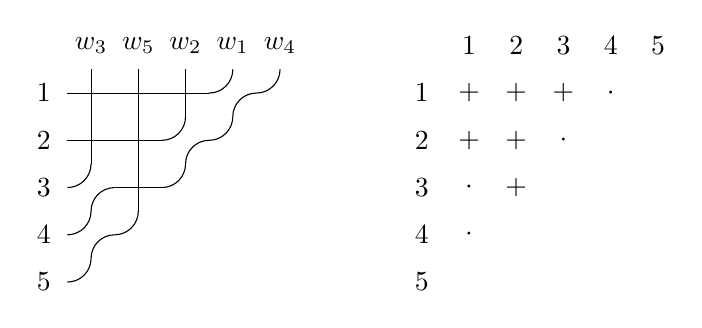
\begin{tikzpicture}[scale=0.3]
\draw (0,-1)--(6,-1);
\draw (6,-1) arc (270:360:1);
\draw (0,-3)--(4,-3);
\draw (4,-3) arc (270:360:1);
\draw (5,-2)--(5,0);
\draw (0,-5) arc(270:360:1);
\draw (1,-4)--(1,0);
\draw (0,-7) arc (270:360:1);
\draw (2,-5) arc (90:180:1);
\draw (2,-5)--(4,-5);
\draw (4,-5) arc (270:360:1);
\draw (6,-3) arc (90:180:1);
\draw (6,-3) arc (270:360:1);
\draw (8,-1) arc (90:180:1);
\draw (8,-1) arc (270:360:1);
\draw (0,-9) arc (270:360:1);
\draw (2,-7) arc (90:180:1);
\draw (2,-7) arc (270:360:1);
\draw (3,-6)--(3,0);
\node at (-1,-1) {1};
\node at (-1,-3) {2};
\node at (-1,-5) {3};
\node at (-1,-7) {4};
\node at (-1,-9) {5};
\node at (1,1) {$w_3$};
\node at (3,1) {$w_5$};
\node at (5,1) {$w_2$};
\node at (7,1) {$w_1$};
\node at (9,1) {$w_4$};
\node at (15,-1) {1};
\node at (15,-3) {2};
\node at (15,-5) {3};
\node at (15,-7) {4};
\node at (15,-9) {5};
\node at (17,1) {1};
\node at (19,1) {2};
\node at (21,1) {3};
\node at (23,1) {4};
\node at (25,1) {5};
\node at (17,-1) {+};
\node at (19,-1) {+};
\node at (21,-1) {+};
\node at (23,-1) {$\cdot$};
\node at (17,-3) {+};
\node at (19,-3) {+};
\node at (21,-3) {$\cdot$};
\node at (17,-5) {$\cdot$};
\node at (19,-5) {+};
\node at (17,-7) {$\cdot$};
\end{tikzpicture}
\caption{An example of an RC-graph for permutation $w=35214$ and of type $(3,2,1,0,0,\ldots)$}
\label{fig:rcex}
\end{figure}

For a piece of notation, for an RC-graph $D$, write $w(D)$ for its permutation and $\alpha(D)$ for its type. Let $\RC(w)$ be the set of all RC-graphs for permutation $w$. And for $\alpha=(\alpha_1,\alpha_2,\ldots)\in\Z_{\geq0}^{\infty}$ with finitely many nonzero positive integer entries, let $x^{\alpha}:=x_1^{\alpha_1}x_2^{\alpha_2}\cdots.$ The following theorem is usually formulated in terms of reduced words.
\begin{theorem}[\cite{billey1993some,fomin1994schubert}]\label{thm:rc}
$\mathfrak{S}_w=\sum_{D\in\RC(w)}x^{\alpha(D)}.$
\end{theorem}
Note that Theorem~\ref{thm:rc} proves a stability property of the Schubert polynomials. Namely, for $w\in S_n$, let $w'$ be its image under the most natural inclusion map $S_n\hookrightarrow S_{n+1}$ by permuting the first $n$ elements. Then $\mathfrak{S}_w=\mathfrak{S}_{w'}$. As a result, from now on, instead of concerning ourselves with $S_n$ where $n$ varies, we will be considering $S_{\infty}$, which is the injective limit of symmetric groups $S_1\hookrightarrow S_2\hookrightarrow S_3\hookrightarrow\cdots$, whose elements are permutations of $\Z_{>0}$ with finitely many non-fixed points. Then $\mathfrak{S}_w$ is well-defined for $w\in S_{\infty}$. 

Local moves on RC-graphs for a fixed permutation are described in~\cite{bergeron1993rc}. A \emph{chute move} $C_{ij}$, can be applied to $D\in\RC(w)$, when the following conditions are satisfied:
\begin{itemize}
\item $(i,j)\in D$, $(i+1,j)\notin D$;
\item $(i,j-m),(i+1,j-m)\notin D$ for some $0<m<j$;
\item $(i,j-k),(i+1,j-k)\in D$ for each $0<k<m$.
\end{itemize}
The resulting RC-graph is $C_{ij}(D)=D\setminus\{(i,j)\}\cup\{(i+1,j-m)\}.$ An example is shown in Figure~\ref{fig:chute}. It is easy to see that if $D\in\RC(w)$ and the above conditions are satisfied, then $C_{ij}(D)\in\RC(w)$. Bergeron and Billey~\cite{bergeron1993rc} also showed that chute moves (and their inverses) connect $\RC(w)$. 
Because of this graphically representation, we will sometimes call an element in $D$ a ``box''. 

\begin{figure}[htb]
\centering
\begin{tikzpicture}[scale=0.4]
\node at (2,0) {$j$-$m$};
\node at (10,0) {$j$};
\node at (0,-2) {$i$};
\node at (0,-4) {$i$+$1$};
\node at (2,-2) {$\cdot$};
\node at (4,-2) {+};
\node at (6,-2) {+};
\node at (8,-2) {+};
\node at (10,-2) {+};
\node at (2,-4) {$\cdot$};
\node at (4,-4) {+};
\node at (6,-4) {+};
\node at (8,-4) {+};
\node at (10,-4) {$\cdot$};
\node at (14,-2) {$\rightarrow$};
\node at (18,-2) {$i$};
\node at (18,-4) {$i$+1};
\node at (20,-2) {$\cdot$};
\node at (22,-2) {+};
\node at (24,-2) {+};
\node at (26,-2) {+};
\node at (28,-2) {$\cdot$};
\node at (20,-4) {+};
\node at (22,-4) {+};
\node at (24,-4) {+};
\node at (26,-4) {+};
\node at (28,-4) {$\cdot$};
\node at (20,0) {$j$-$m$};
\node at (28,0) {$j$};
\end{tikzpicture}
\caption{A chute move}
\label{fig:chute}
\end{figure}


\subsection{D-pairing}
Define the \emph{D-pairing} on (each graded component of) the space of polynomials in infinitely many variables $\Q[x_1,x_2,\ldots]$ by
\[
(f,g)_D:=\CT(f(\partial/\partial x)\cdot g(x))
\]
where $\CT$ stands for constant term. We see that the monomial basis of $\Q[x_1,x_2,\ldots]$ form an orthogonal basis with respect to the D-pairing such that $(x^{\alpha},x^{\alpha})_D=\alpha_1!\alpha_2!\cdots$ and thus the D-pairing is symmetric and non-degenerate.

As the name suggests, dual Schubert polynomials are dual to the Schubert polynomials with respect to the D-pairing.
\begin{theorem}[Corollary~12.3 of~\cite{postnikov2009chains}]\label{thm:dual}
The sets of polynomials $\{\mathfrak{S}_w\}_{w\in S_{\infty}}$ and $\{\D_w\}_{w\in S_{\infty}}$ form a dual basis w.r.t.\ the D-pairing. In other words, both $\{\mathfrak{S}_w\}_{w\in S_{\infty}}$ and $\{\D_w\}_{w\in S_{\infty}}$ are basis of $\Q[x_1,x_2,\ldots]$ and $(\mathfrak{S}_w,\D_u)=\delta_{w,u}$ where $\delta$ is the Kronecker delta. 
\end{theorem}
Theorem~\ref{thm:dual} easily implies the following lemma, which is our main tool.
\begin{lemma}\label{lem:basis}
If $f\in\Q[x_1,x_2,\ldots]$ satisfies $(f,\mathfrak{S}_u)_D=\delta_{w,u}$ for all $u\in S_{\infty}$, then $f=\D_w$.
\end{lemma}

\section{Main Theorem and Proof}\label{sec:main}
In this section, we resolve Conjecture 16.1 of~\cite{postnikov2009chains}. We will be mainly following notations of~\cite{postnikov2009chains}, but we remark that there are some errors in the original formulation. Recall that the \emph{(Lehmer) code} of a permutation is defined to be
\[
\code(w)_i:=\#\{j>i:w(j)<w(i)\}.
\]
Permutations can be reconstructed from their codes.
\begin{defi}
We say that a permutation $w$ is \emph{special}, if its code has the form
\[
\code(w)=(n,*,n-1,*,\ldots,*,2,*,1,0,0,\ldots)
\]
where $*$ is either a single 0 or empty.
\end{defi}
For a special permutation $w$, write $\code(w)=(c_1,c_2,\ldots,0,0,\ldots)$. Let $c_1=n$ and let $a_1<a_2<\cdots<a_k$ be the indices such that $c_{a_i}=0$ and $c_{a_i-1}>0$. We can then view $w$ as a permutation in $S_{n+k}\hookrightarrow S_{\infty}$. 

Define
\[
g_{\delta}(y_1,\ldots,y_m)=\sum_{u\in S_m}(-1)^{\ell(w_0)-\ell(u)}y_1^{u(1)}\cdots y_m^{u(m)}=y_1\cdots y_m\prod_{1\leq i<j\leq m}(y_i-y_j).
\]
An $n$-element subset $J=\{j_1,\ldots,j_n\}$ of $\{1,2,\ldots,n+k\}$ is said to be \emph{valid} (with respect to $w$) if
\[
\#(J\cap\{a_{i-1}+1,a_{i-1}+2,\ldots,a_i-1,a_i\})=a_i-a_{i-1}-1
\]
for all $1\leq i\leq k$. If $J$ is a valid set, let $\epsilon_J=(-1)^{d_J}$ where
\[
d_J=(j_1+\cdots+j_n)-\binom{n+k+1}{2}+(a_1+\cdots+a_k)
\]
which gives sign 1 to the valid subset $L$ with the smallest element sum.
\begin{theorem}[Conjecture 16.1 of~\cite{postnikov2009chains}]\label{thm:main}
Let $w$ be special as above. Then
\[
\D_w=\frac{1}{1!2!\cdots n!}\sum_{J=\{j_1,\ldots,j_n\}\text{ valid}}\epsilon_J g_{\delta}(x_{j_1},x_{j_2},\ldots,x_{j_n}).
\]
\end{theorem}
Before proving Theorem~\ref{thm:main}, let us utilize chute moves defined in Section~\ref{sec:intro} and define a slightly more complicated move on RC-graphs. We say that a \emph{flip move} $F_{i,j}$ can be applied to $D\in\RC(w)$ if $(i,j)\notin D$. As in a chute move, we will only change row $i$ and row $i+1$. The procedure of such a move is explained as follows. Let us first ``ignore'' columns $p$ such that $(i,p),(i+1,p)\in D$, meaning that these entries $(i,p),(i+1,p)$ will still stay in $F_{i,j}(D)$ after the flip. Notice that in a chute move, such columns are always fixed. Consider all boxes $(q_1,p)\in D$ such that $(q_2,p)\notin D$ where $\{q_1,q_2\}=\{i,i+1\}$. We call these boxes \emph{single} and connect them by the following rules:
\begin{itemize}
\item connect $(q,p)$ and $(q,p')$ if for all $k\in \{p+1,\ldots,p'-1\}$, $(i,k),(i+1,k)\in D$;
\item connect $(i+1,p)$ and $(i,p')$ if for all but one $k\in\{p+1,\ldots,p'-1\}$, $(i,k),(i+1,k)\in D$ with the exception that for one $k'\in \{p+1,\ldots,p'-1\}$, $(i,k'),(i+1,k')\notin D$.
\end{itemize}
These rules divide all such boxes into chains. Each chain consists of boxes $(i+1,q_1),\ldots,(i+1,q_a),(i,q_{a+2}),\ldots,(i,q_{a+b+1})$ with $j\leq q_1<\cdots<q_{a+b}$ where the index $q_{a+1}$ is such that $(i,q_{a+1}),(i+1,q_{a+1})\notin D$, and $a,b\geq0$. For the flip move $F_{i,j}$, we change (remove then add) these boxes to $(i+1,q_1),\ldots,(i+1,q_b),(i,q_{b+2}),\ldots,(i,q_{a+b+1}).$ For such a chain, this flip is in fact $b-a$ chute moves from left to right applied to the middle $b-a$ elements of $D$ if $a\leq b$, or $a-b$ inverse chute moves if $a\geq b$. An example is shown in Figure~\ref{fig:flip}.
\begin{figure}[h!]
\centering
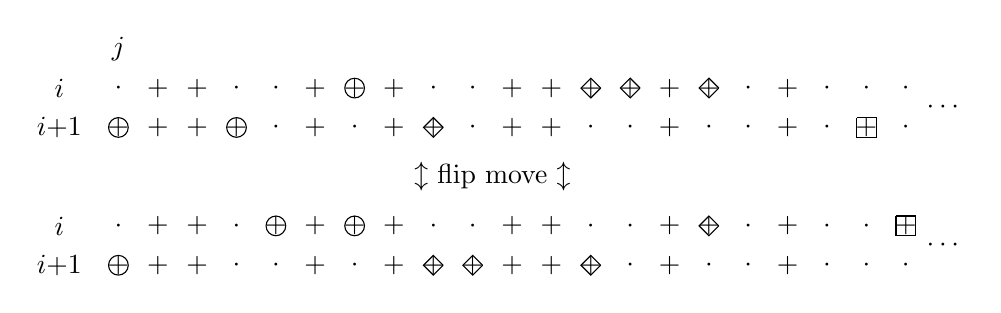
\begin{tikzpicture}[scale=0.25]
\node at (2,2) {$j$};
\node at (-1,0) {$i$};
\node at (-1,-2) {$i$+1};
\node at (2,0) {$\cdot$};
\node at (2,-2) {+};
\node at (4,0) {+};
\node at (4,-2) {+};
\node at (6,0) {+};
\node at (6,-2) {+};
\node at (8,0) {$\cdot$};
\node at (8,-2) {+};
\node at (10,0) {$\cdot$};
\node at (10,-2) {$\cdot$};
\node at (12,0) {+};
\node at (12,-2) {+};
\node at (14,0) {+};
\node at (14,-2) {$\cdot$};
\node at (16,0) {+};
\node at (16,-2) {+};
\node at (18,0) {$\cdot$};
\node at (18,-2) {+};
\node at (20,0) {$\cdot$};
\node at (20,-2) {$\cdot$};
\node at (22,0) {+};
\node at (22,-2) {+};
\node at (24,0) {+};
\node at (24,-2) {+};
\node at (26,0) {+};
\node at (26,-2) {$\cdot$};
\node at (28,0) {+};
\node at (28,-2) {$\cdot$};
\node at (30,0) {+};
\node at (30,-2) {+};
\node at (32,0) {+};
\node at (32,-2) {$\cdot$};
\node at (34,0) {$\cdot$};
\node at (34,-2) {$\cdot$};
\node at (36,0) {+};
\node at (36,-2) {+};
\node at (38,0) {$\cdot$};
\node at (38,-2) {$\cdot$};
\node at (40,0) {$\cdot$};
\node at (40,-2) {+};
\node at (42,0) {$\cdot$};
\node at (42,-2) {$\cdot$};
\node at (44,-1) {$\cdots$};
\draw (2.5,-2) arc (0:360:0.5);
\draw (8.5,-2) arc (0:360:0.5);
\draw (14.5,0) arc (0:360:0.5);
\draw (18.5,-2)--(18,-2.5)--(17.5,-2)--(18,-1.5)--(18.5,-2);
\draw (26.5,0)--(26,-0.5)--(25.5,0)--(26,0.5)--(26.5,0);
\draw (28.5,0)--(28,-0.5)--(27.5,0)--(28,0.5)--(28.5,0);
\draw (32.5,0)--(32,-0.5)--(31.5,0)--(32,0.5)--(32.5,0);
\draw (39.5,-1.5)--(40.5,-1.5)--(40.5,-2.5)--(39.5,-2.5)--(39.5,-1.5);

\node at (-1,-7) {$i$};
\node at (-1,-9) {$i$+1};
\node at (2,-7) {$\cdot$};
\node at (2,-9) {+};
\node at (4,-7) {+};
\node at (4,-9) {+};
\node at (6,-7) {+};
\node at (6,-9) {+};
\node at (8,-7) {$\cdot$};
\node at (8,-9) {$\cdot$};
\node at (10,-7) {+};
\node at (10,-9) {$\cdot$};
\node at (12,-7) {+};
\node at (12,-9) {+};
\node at (14,-7) {+};
\node at (14,-9) {$\cdot$};
\node at (16,-7) {+};
\node at (16,-9) {+};
\node at (18,-7) {$\cdot$};
\node at (18,-9) {+};
\node at (20,-7) {$\cdot$};
\node at (20,-9) {+};
\node at (22,-7) {+};
\node at (22,-9) {+};
\node at (24,-7) {+};
\node at (24,-9) {+};
\node at (26,-7) {$\cdot$};
\node at (26,-9) {+};
\node at (28,-7) {$\cdot$};
\node at (28,-9) {$\cdot$};
\node at (30,-7) {+};
\node at (30,-9) {+};
\node at (32,-7) {+};
\node at (32,-9) {$\cdot$};
\node at (34,-7) {$\cdot$};
\node at (34,-9) {$\cdot$};
\node at (36,-7) {+};
\node at (36,-9) {+};
\node at (38,-7) {$\cdot$};
\node at (38,-9) {$\cdot$};
\node at (40,-7) {$\cdot$};
\node at (40,-9) {$\cdot$};
\node at (42,-7) {+};
\node at (42,-9) {$\cdot$};
\node at (44,-8) {$\cdots$};
\draw (2.5,-9) arc (0:360:0.5);
\draw (10.5,-7) arc (0:360:0.5);
\draw (14.5,-7) arc (0:360:0.5);
\draw (18.5,-9)--(18,-9.5)--(17.5,-9)--(18,-8.5)--(18.5,-9);
\draw (20.5,-9)--(20,-9.5)--(19.5,-9)--(20,-8.5)--(20.5,-9);
\draw (26.5,-9)--(26,-9.5)--(25.5,-9)--(26,-8.5)--(26.5,-9);
\draw (32.5,-7)--(32,-7.5)--(31.5,-7)--(32,-6.5)--(32.5,-7);
\draw (41.5,-6.5)--(42.5,-6.5)--(42.5,-7.5)--(41.5,-7.5)--(41.5,-6.5);
\node at (21,-4.5) {$\updownarrow$ flip move $\updownarrow$};
\end{tikzpicture}
\caption{An example of a flip move, where different chains of single boxes are labeled by different shapes.}
\label{fig:flip}
\end{figure}

A few simple facts ensure that our flip move is well-defined. First, there is never a configuration in the form of $(i+1,p),(i,p')\in D$, $(i,p),(i+1,p')\notin D$, and for all $p<k<p'$, $(i,k),(i+1,k)\in D$, since otherwise, the RC-graph is not reduced. This fact guarantees that we can indeed partition all single boxes into chains as described above, and that each chain lie ``strictly'' to the left or right of each other. Second, the condition $(i,j)\notin D$ is essential since otherwise, if the leftmost chain contains $(i,j)$, during our flip move which may contain a chute move at $(i,j)$, we would need to require certain boxes whose column indices are less than $j$ to be not in $D$. Such condition is inconvenient since $j$ might even be 1.

An important property of the flip move defined above, suggested by its name, is that $F_{i,j}(F_{i,j}(D))=D$ when $(i,j)\notin D$. 

We are now ready to prove Theorem~\ref{thm:main}.
\begin{proof}[Proof of Theorem~\ref{thm:main}]
Let 
\[
f:=\frac{1}{1!2!\cdots n!}\sum_{J=\{j_1,\ldots,j_n\}\text{ valid}}\epsilon_J g_{\delta}(x_{j_1},x_{j_2},\ldots,x_{j_n})
\]
be the desired expression. By Lemma~\ref{lem:basis}, it suffices to show that $(f,\mathfrak{S}_u)_D=\delta_{wu}$, for all $u\in S_{\infty}$.

Fix $u\in S_{\infty}$. To use the D-pairing, we expand both $f$ and $\mathfrak{S}_u$ as sums of monomials. By Theorem~\ref{thm:rc}, $\mathfrak{S}_u=\sum_{\alpha} c_{u,\alpha}x^{\alpha}$, where $c_{u,\alpha}$ is the number of RC-graphs for permutation $u$ and of type $\alpha$. To compute $(f,\mathfrak{S}_u)_D$, we only need to pay attention to the number of RC-graphs of \emph{special} types $\alpha$, which means that $x^{\alpha}$ appear in the expansion of $f$. More explicitly, by definition of $g_{\delta}$, we know that for $\alpha$ being a special type, the nonzero entries of $\alpha_1,\alpha_2,\ldots$ are precisely $1,2,\ldots,n$ and in order for $x^{\alpha}$ to appear in some $g_{\delta}(x_{j_1},\ldots,x_{j_n})$ with $J=\{j_1,\ldots,j_n\}$ valid, the number of zeros among $\alpha_{a_{i-1}+1},\ldots,\alpha_{a_i}$ is exactly 1 for $i=1,\ldots,k$, and $\alpha_j=0$ for $j>n+k$. From now on, for a special type $\alpha$, we view it as an array of $n+k$ numbers, instead of an infinite array. Let $\RC_s(u)$ be the set of all RC-graphs for permutation $u$ and of special types. Moreover, for each $D\in\RC_s(u)$, we can associate a sign $\wt(\alpha)$ to $D$ based on its type $\alpha$ according to $f$. It is possible to write down explicitly the sign, but for our purpose, the following rules are more useful:
\begin{enumerate}
\item\label{proof_theo2.2_prem1} If $\alpha=\code(w)$, $\wt(\alpha)=1$;
\item\label{proof_theo2.2_prem2} If $\alpha'$ is obtained from $\alpha$ by switching two nonzero entries, then $\wt(\alpha')=-\wt(\alpha)$;
\item\label{proof_theo2.2_prem3} If $\alpha'$ is obtained from $\alpha$ by switching a zero with its adjacent nonzero entry such that $\alpha'$ remains special, then $\wt(\alpha')=-\wt(\alpha)$.
\end{enumerate}
Let's justify the rules here. For~\eqref{proof_theo2.2_prem1}, when $\alpha=\code(w)$, the corresponding valid set $J$ satisfies that $J\supset\{a_{i-1}+1,\ldots,a_i-1\}$ so $(j_1+\cdots+j_n)+(a_1+\cdots+a_k)=1+2+\cdots+(n+k)$ and as a result, $d_J=0$, $\epsilon_J=1$. And as the nonzero entries of $\alpha$ are increasing, the sign of $\alpha$ is the same as $\epsilon_J$. Rule~\eqref{proof_theo2.2_prem2} follows from the fact that a transposition changes the sign of a permutation. For~\eqref{proof_theo2.2_prem3}, let $J$ and $J'$ be the corresponding valid sets for $\alpha$ and $\alpha'$ respectively. As $J$ and $J'$ differ by an adjacent pair of numbers, $d_J$ and $d_J'$ differ by 1 so their signs are different. But the permutations (in the expansion of $g_{\delta}$) associated with $\alpha$ and $\alpha'$ are the same so in the end, $\wt(\alpha')=-\wt(\alpha)$.

Since for a special type $\alpha$, $(x^{\alpha},x^{\alpha})_D=1!2!\cdots n!$, we can interpret $(f,\mathfrak{S}_u)_D$ as a weighted sum of RC-graphs in $\RC_s(u)$, where the weights are $\pm1$ explained above.

For example, if $w=41532$ is special, then $\code(w)=(3,0,2,1,0)$. There are a total number of 36 special types: 2 possibilities for the position of the first zero that appears as either $\alpha_1$ or $\alpha_2$, 3 possibilities for the position of the second zero, and 6 possibilities for the permutation of $3,2,1$. As for the weights, we have $\wt(3,0,2,1,0)=1$, $\wt(0,3,2,1,0)=-1$, $\wt(0,1,2,3,0)=1$, $\wt(0,1,2,0,3)=-1$, etc. 

Our strategy is using flip moves to pair up RC-graphs of special types with different signs. We will do this in steps. Let $I=\{1,2,\ldots,n+k\}\setminus\{a_1,a_2,\ldots,a_k\}$ be the index set of positions where $\code(w)$ is nonzero. We say that $D\in\RC_s(u)$ is 1-\emph{flippable}, if there exists $i\in I$ such that $(i,1)\notin D$. For each 1-flippable RC-graph $D\in\RC_s(u)$, we can pair it up with $F_{i_0,1}(D)$ where $i_0$ is the smallest index in $I$ such that $(i_0,1)\notin D$. Notice that in this case, $D'=F_{i_0,1}(D)$ is also 1-flippable because of the existence of $i_0$ and that $i_0$ is the smallest index in $I$ such that $(i_0,1)\notin D'$ as well. Moreover, $\alpha(D')$ can be obtained from $\alpha(D)$ by switching the $i_0^{th}$ entry and $(i_0+1)^{th}$ entry. Thus, $D'\in\RC_s(u)$ and $D'$ and $D$ have opposite signs. As a result, $F_{*,1}$ is a sign-reversing involution on the set of all 1-flippable RC-graphs in $\RC_s(u)$. By taking out all such graphs, we are left with RC-graphs that are not 1-flippable. Denote such set as $\RC_{s'}(u)$. 

Notice that for $D\in\RC_{s'}(u)$ and $\alpha=\alpha(D)$, since $(i_0,1)\in D$ for all $i_0\in I$, we know that $\alpha_{a_i}=0$ for $i=1,\ldots,k$. Our next step will be a generalization to the above procedure.

We say that $D\in\RC_{s'}(u)$ is $j$-\emph{flippable}, for some $j\geq1$, if there exists $i\in I$ satisfying the following condition:
\begin{enumerate}
\item\label{proof_theo2.2_deux1} If $a_{t-1}+1\leq i<a_t-1$ for some $t=1,\ldots,k$ (by convention $a_{0}=0$), we require $j\geq t$ and $\{(i,1),(i,2),\ldots,(i,j-t+1)\}\cap D$ has the same cardinality as $\{(i+1,1),(i+1,2),\ldots,(i+1,j-t)\}\cap D$;
\item\label{proof_theo2.2_deux2} If $i=a_t-1$ for some $t$, we require $j\geq t$ and $\{(i,1),(i,2),\ldots,(i,j-t+1)\}\cap D$ has the same cardinality as $\{(i+2,1),(i+2,2),\ldots,(i+2,j-t-1)\}\cap D$.
\end{enumerate}
We say that $D\in\RC_{s'}(u)$ is $j$-flippable at row $i\in I$ if such condition is satisfied, and that $D$ is $j$-flippable at minimum row $i$ if $D$ is $j$-flippable and that $i$ is the smallest index such that $D$ is $j$-flippable at $i$. We have abused the notion of 1-flippable but as our original definition of 1-flippable implies the new-defined version, we see that each $D\in\RC_{s'}(u)$ is not 1-flippable so there won't be a problem.

Fixing $i_0\in I$ and $j$, we are now going to use flip moves to construct a sign-reversing involution on all RC-graphs in $\RC_{s'}(u)$ that are not $j'$-flippable for every $j'<j$ and are $j$-flippable at minimum row $i_0$. Let such set of RC-graphs be $\RC_{s'}^{i_0,j}$. There are two cases.


\let\oldthecdrthm\thecdrthm
\renewcommand{\thecdrthm}{(\arabic{cdrthm})}
\setcounter{cdrthm}{0}
\begin{enonce}[remark]{Case}\label{case1}
 $a_{t-1}+1\leq i_0<a_t-1$ for some $t=1,\ldots,k$. When $j'=t$, $\{(i_0,1),\ldots,(i_0,j'-t+1)\}\cap D=\{(i_0,1)\}$ which has cardinality 1 and $\{(i_0+1,1),\ldots,(i_0+1,j'-t)\}\cap D=\emptyset$ which has cardinality 0. If $j'$ increases by 1, the cardinality of $\{(i_0,1),\ldots,(i_0,j'-t+1)\}\cap D$ increases by 1 or 0 and so does the cardinality of $\{(i_0+1,1),\ldots,(i_0+1,j'-t)\}\cap D$. Since $D$ is not $j'$-flippable for all $j'<j$, the cardinality of the first set is always greater than the cardinality of the second set. As $D$ is $j$-flippable at row $i_0$, we deduce that $(i_0,j-t+1)\notin D$. This allows us to apply $F_{i_0,j-t+1}$ to $D$. We are going to verify in a moment that $F_{i_0,j-t+1}(D)\in\RC_{s'}^{i_0,j}$.
\end{enonce}

\begin{enonce}[remark]{Case}\label{case2}
%\textbf{Case (2)}: 
$i_0=a_t-1$ for some $t=1,\ldots,k$. With the same argument, $(i_0,j-t+1)\notin D$. We are now going to apply a modified flip move $F_{i_0,j-t+1}'$ to $D$. As row $i_0+1=a_t$ of $D$ is completely empty, and recall that $(i,j)\in D$ represents the simple transposition $s_{i+j-1}$ in the corresponding reduced decomposition, we can move every box with row index at least $i_0+2$ in the direction of $(-1,1)$, without changing the corresponding permutation $u$ (and its reduced decomposition). Call this RC-graph $\bar D$. Apply $F_{i_0,j-t+1}$ to $\bar D$ to obtain $\bar D'$. Then move every box with row index at least $i_0+1$ in the direction of $(1,-1)$ to finally arrive at $D'$. Write $F_{i_0,j-t+1}'(D)=D'$. An example is shown in Figure~\ref{fig:flipmodi}.

\begin{figure}[h!]
\centering
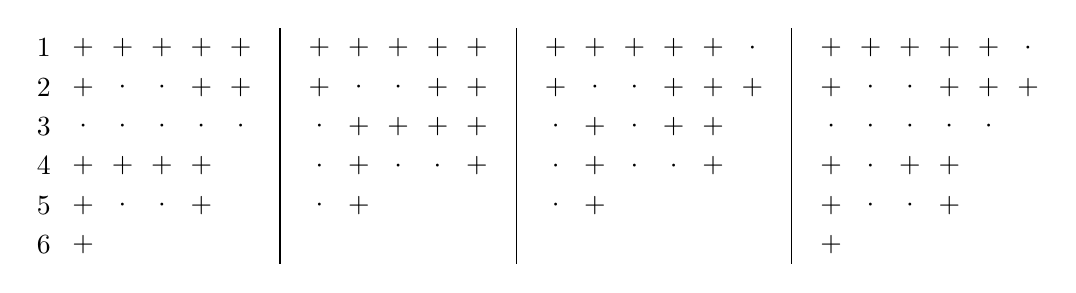
\begin{tikzpicture}[scale=0.25]
\node at (0,0) {1};
\node at (0,-2) {2};
\node at (0,-4) {3};
\node at (0,-6) {4};
\node at (0,-8) {5};
\node at (0,-10) {6};
\node at (2,0) {+};
\node at (4,0) {+};
\node at (6,0) {+};
\node at (8,0) {+};
\node at (10,0) {+};
\node at (2,-2) {+};
\node at (4,-2) {$\cdot$};
\node at (6,-2) {$\cdot$};
\node at (8,-2) {+};
\node at (10,-2) {+};
\node at (2,-4) {$\cdot$};
\node at (4,-4) {$\cdot$};
\node at (6,-4) {$\cdot$};
\node at (8,-4) {$\cdot$};
\node at (10,-4) {$\cdot$};
\node at (2,-6) {+};
\node at (4,-6) {+};
\node at (6,-6) {+};
\node at (8,-6) {+};
\node at (2,-8) {+};
\node at (4,-8) {$\cdot$};
\node at (6,-8) {$\cdot$};
\node at (8,-8) {+};
\node at (2,-10) {+};
\draw (12,1)--(12,-11);

\node at (14,0) {+};
\node at (16,0) {+};
\node at (18,0) {+};
\node at (20,0) {+};
\node at (22,0) {+};
\node at (14,-2) {+};
\node at (16,-2) {$\cdot$};
\node at (18,-2) {$\cdot$};
\node at (20,-2) {+};
\node at (22,-2) {+};
\node at (14,-4) {$\cdot$};
\node at (16,-4) {+};
\node at (18,-4) {+};
\node at (20,-4) {+};
\node at (22,-4) {+};
\node at (14,-6) {$\cdot$};
\node at (16,-6) {+};
\node at (18,-6) {$\cdot$};
\node at (20,-6) {$\cdot$};
\node at (22,-6) {+};
\node at (14,-8) {$\cdot$};
\node at (16,-8) {+};
\draw (24,1) -- (24,-11);

\node at (26,0) {+};
\node at (28,0) {+};
\node at (30,0) {+};
\node at (32,0) {+};
\node at (34,0) {+};
\node at (36,0) {$\cdot$};
\node at (26,-2) {+};
\node at (28,-2) {$\cdot$};
\node at (30,-2) {$\cdot$};
\node at (32,-2) {+};
\node at (34,-2) {+};
\node at (36,-2) {+};
\node at (26,-4) {$\cdot$};
\node at (28,-4) {+};
\node at (30,-4) {$\cdot$};
\node at (32,-4) {+};
\node at (34,-4) {+};
\node at (26,-6) {$\cdot$};
\node at (28,-6) {+};
\node at (30,-6) {$\cdot$};
\node at (32,-6) {$\cdot$};
\node at (34,-6) {+};
\node at (26,-8) {$\cdot$};
\node at (28,-8) {+};
\draw (38,1) -- (38,-11);

\node at (40,0) {+};
\node at (42,0) {+};
\node at (44,0) {+};
\node at (46,0) {+};
\node at (48,0) {+};
\node at (50,0) {$\cdot$};
\node at (40,-2) {+};
\node at (42,-2) {$\cdot$};
\node at (44,-2) {$\cdot$};
\node at (46,-2) {+};
\node at (48,-2) {+};
\node at (50,-2) {+};
\node at (40,-4) {$\cdot$};
\node at (42,-4) {$\cdot$};
\node at (44,-4) {$\cdot$};
\node at (46,-4) {$\cdot$};
\node at (48,-4) {$\cdot$};
\node at (40,-6) {+};
\node at (42,-6) {$\cdot$};
\node at (44,-6) {+};
\node at (46,-6) {+};
\node at (40,-8) {+};
\node at (42,-8) {$\cdot$};
\node at (44,-8) {$\cdot$};
\node at (46,-8) {+};
\node at (40,-10) {+};
\end{tikzpicture}
\caption{An example of the sign reversing involution $F_{i_0,j-t+1}'$ where $\code(w)=(5,4,0,3,2,1,0)$, $i_0=2$, $j=3$. From left to right: $D$, which is not 1-flippable or 2-flippable, but is 3-flippable at minimum row 2; $\bar D$, which is obtained from $D$ by moving row 4,5,6 via $(-1,1)$; $\bar D'=F_{2,3}(\bar D)$; $D'$, which is obtained from $\bar D'$ by moving row 4,5,6 via $(1,-1)$.}
\label{fig:flipmodi}
\end{figure}
\end{enonce}
\let\thecdrthm\oldthecdrthm
\setcounter{cdrthm}{2}

We are now going to show that such construction indeed provides a sign-reversing involution. Consider Case (1) first. Recall $D\in\RC_{s'}^{i_0,j}$ and $D'=F_{i_0,j-t+1}(D)$, which only changes row $i_0$ and $i_0+1$ after column $j-t$. Therefore, for each $j'<j$, for $a_{t-1}+1\leq i<a_t-1$, $\{(i,1),\ldots,(i,j'-t+1)\}\cap D=\{(i,1),\ldots,(i,j'-t+1)\}\cap D'$, $\{(i+1,1),\ldots,(i+1,j'-t)\}\cap D=\{(i+1,1),\ldots,(i+1,j'-t)\}\cap D'$, and for $i=a_t-1$, $\{(i,1),\ldots,(i,j'-t+1)\}\cap D=\{(i,1),\ldots,(i,j'-t+1)\}\cap D'$, $\{(i+2),\ldots,(i+2,j'-t-1)\}\cap D=\{(i+2),\ldots,(i+2,j'-t-1)\}\cap D'$. So $D'$ is not $j'$-flippable. Moreover, the existence of $i_0$ says that $D'$ is $j$-flippable at row $i_0$. With the same reason that a flip move only changes row $i_0$ and $i_0+1$ after column $j-t$, we know that $D'$ is $j$-flippable at minimum row $i_0$. So $D'\in\RC_{s'}^{i_0,j}$. As for its type, by definition of a flip move, we know that $\{(i_0,j-t+2),(i_0,j-t+3),\ldots\}\cap D$ has the same cardinality as $\{(i_0+1,j-t+1),(i_0+1,j-t+2),\ldots\}\cap D'$ and since the cardinality of $\{(i_0,1),\ldots,(i_0,j-t+1)\}\cap D$ equals the cardinality of $\{(i_0+1,1),\ldots,(i_0+1,j-t)\}\cap D'$, $\alpha(D)_{i_0}=\alpha(D')_{i_0+1}$. Similarly, $\alpha(D)_{i_0+1}=\alpha(D')$ so $\alpha(D')$ is obtained from $\alpha(D)$ by switching the $i_0^{th}$ entry with $(i_0+1)^{th}$ entry. They have different signs. In fact, Case~\ref{case2} can be unified to Case~\ref{case1} by moving elements in row $i\in I$ of $D$ by $(-t,t)$ where $a_{t-1}<i<a_t$, as in the definition of the modified flip move $F_{i_0,j-t+1}'$, since row $a_t$'s are all empty. Then the same arguments work.

Finally, we are left with special RC-graphs that are not $j$-flippable for all $j$. We claim that there is exactly one such RC-graph $D_0$ and that it is for the permutation $w$ and of type $\alpha=\code(w)$. This RC-graph is known as the \emph{bottom RC-graph} for $w$ (see~\cite{bergeron1993rc}). First, for two consecutive rows $i,i+1\in I$, $\{(i,1),\ldots,(i,j-t+1)\}\cap D$ has different cardinality than $\{(i+1,1),\ldots,(i+1,j-t)\}\cap D$. But when $j$ increases by 1, both sets increase by 0 or 1 and since $(i,1)\in D$, we must have that the cardinality of the first set stays always above the cardinality of the second. When $j$ is sufficiently large, we deduce $\alpha_i>\alpha_{i+1}$. Similarly, $\alpha_i>\alpha_{i+2}$ for $i=a_t-1$. Thus, the nonzero entries of $\alpha$ are decreasing, and thus $\alpha=\code(w)$. Next, we use backwards induction to show that $(i,1),(i,2),\ldots,(i,\alpha_i)\in D$, $i\in I$. As we already know $(i,1)\in D$ for all $i\in I$, the base case $i=a_k-1$ is established. For a general $i$, if $a_{t-1}+1\leq i< a_t-1$, then $i+1\in I$ and $(i+1,1),\ldots,(i+1,\alpha_{i+1})\in D$. The non-flippable property directly implies that $(i,1),\ldots,(i,\alpha_{i+1}+1)\in D$ so we are done as $\alpha_{i+1}+1=\alpha_i$. If $i=a_t-1$ for some $t$, then $i+1\notin I$, $i+2\in I$, $\alpha_{i}=\alpha_{i+2}+1$. The non-flippable property implies that the cardinality of $\{(i,1),\ldots,(i,\alpha_i+1)\}\cap D$ is $\alpha_i$ so we just need to figure out which box among $(i,1),\ldots,(i,\alpha_i+1)$ is not in $D$. If $(i,k)\notin D$ for some $k\leq\alpha_i$, then the two strands emanating up and right from $(i+2,k-1)$ meet again at $(i,\alpha_{i}+1)$ (Figure~\ref{fig:indNon}), meaning $D$ is not reduced. Thus, $(i,1),\ldots,(i,\alpha_i)\in D$ and our induction step goes through. This RC-graph $D$ is indeed the bottom RC-graph for $w$, which is reduced and corresponds to $w$ (see~\cite{bergeron1993rc}).
\end{proof}

\begin{figure}[h!]
\centering
\begin{tikzpicture}[scale=0.4]
\node at (0,-2) {$i$};
\node at (0,-4) {$i$+1};
\node at (0,-6) {$i$+2};
\node at (8,0) {$j$};
\node at (12,0) {$\alpha_i$+1};
\node at (2,-2) {+};
\node at (4,-2) {+};
\node at (6,-2) {+};
\node at (8,-2) {$\cdot$};
\node at (10,-2) {+};
\node at (12,-2) {+};
\node at (2,-4) {$\cdot$};
\node at (4,-4) {$\cdot$};
\node at (6,-4) {$\cdot$};
\node at (8,-4) {$\cdot$};
\node at (10,-4) {$\cdot$};
\node at (2,-6) {+};
\node at (4,-6) {+};
\node at (6,-6) {+};
\node at (8,-6) {+};
\draw (12,-3)--(12,-2)--(9,-2);
\draw (9,-2) arc (90:180:1);
\draw (7,-4) arc (270:360:1);
\draw (7,-4) arc (90:180:1);
\draw (6,-5)--(6,-6)--(9,-6);
\draw (11,-4) arc (270:360:1);
\draw (11,-4) arc (90:180:1);
\draw (9,-6) arc (270:360:1);
\end{tikzpicture}
\caption{A configuration that is not reduced}
\label{fig:indNon}
\end{figure}

Let's now look at a slight generalization to Theorem~\ref{thm:main}. Suppose that we have positive integers $0<a_1<b_1<a_2<b_2<\cdots<a_k<b_k$ and let $n=\sum_{i=1}^k(b_i-a_i)$. We say that an $n$-element subset $J$ is \emph{valid} with respect to $a,b$ if $\#(J\cap \{a_i,a_i+1,\ldots,b_i\})=b_i-a_i$ for every $i$. Notice that the setting of Theorem~\ref{thm:main} is a special case where $a_{i}-b_{i-1}=1$ for $i=1,\ldots,k$ and $b_{0}=0$ by convention. If $J=\{j_1,\ldots,j_n\}$ is valid, let $\epsilon_J=(-1)^{d_J}$ where 
\[
d_J=(j_1+\cdots+j_n)-\left(\sum_{i=1}^k(a_i+\cdots+(b_i-1))\right).
\]

\begin{theorem}\label{thm:gen}
Use notations as above, 
\[
\frac{1}{1!2!\cdots n!}\epsilon_Jg_{\delta}(x_{j_1},\ldots,x_{j_n})=\sum_{w\in S_{b_k}}m_w\D_w,
\]
where $m_w$'s are non-negative integers.
\end{theorem}
\begin{proof}
The proof strategy is exactly the same as the proof for Theorem~\ref{thm:main}. So we will skip repeated details and provide a sketch here. Let $f$ be the LHS of the theorem statement and $(f,\mathfrak{S}_w)_D$ can be viewed as a weighted sum of RC-graphs of special types for permutation $w$. Likewise, we can define the notion of $j$-flippable RC-graphs and apply (modified) flip moves. The only difference is that instead of moving latter rows $(-1,1)$ to bypass one empty row, we will need to move $(a_{t+1}-b_t)*(-1,1)$ this time. But the principal of ignoring empty rows remains the same. 

In the end, we are left with non-flippable RC-graphs. All of them are of the same type $\alpha$, which takes on values $n,n-1,\ldots,2,1$ at indices $a_1,\ldots,b_1-1,a_2,\ldots,b_2-1,\ldots,a_k,\ldots,b_k-1$ and 0 elsewhere. The weight of $\alpha$ is 1. Let $D$ be such an RC-graph and let $I=\bigcup_{t=1}^k\{a_t,\ldots,b_t-1\}$. We have $(b_k-1,1)\in D$. Then, we use backwards induction on $i$ to show that $(i,j)\notin D$ if $i+j>b_k$. The base case $i=b_k-1$ is established. Moreover, this claim is trivial if $i\notin I$. For a general $i$, let $i'$ be the smallest element greater than $i$ in $I$. By the non-flippable property of $D$, $\{(i,1),\ldots,(i,b_k-i)\}\cap D$ has greater cardinality than $\{(i',1),\ldots,(i',b_k-i')\}\cap D$, which is $\alpha_{i'}$ by induction hypothesis. As $\alpha_i=\alpha_{i'}+1$, we know that $\{(i,1),\ldots,(i,b_k-i)\}\cap D$ must have cardinality $\alpha_i$ so there cannot be more boxes in $i^{th}$ row after $b_k-i$. The induction step goes through. Thus, the decomposition of the permutation of $D$ uses only $s_i$ for $i<b_k$, meaning that the permutation lies in $S_{b_k}$ as desired.
\end{proof}
\longthanks{The author thanks Alex Postnikov and Richard Stanley for helpful conversations.}


\bibliographystyle{amsplain-ac}
\bibliography{ALCO_Gao_266}
\end{document}
